\documentclass{article}
\usepackage[utf8]{inputenc}
\usepackage{amsmath}
\usepackage{amssymb}
\usepackage{graphicx}
\usepackage{hyperref}
\usepackage{tikz}
\usepackage{pgfplots}
\usepackage{float}
\usepackage{listings}
\usepackage{color}
\usepackage{bbm}
\title{Reinforcement Learning - Exercise 1 - Solution}
\author{Jonathan Schnitzler}
\date{\today}
\begin{document}
\maketitle
\section{Multi-Armed Bandits}

\subsection*{Task 1a)}

Since there are only two actions it doesn't mind whether the optimal action is already found, it is always guessing with a probability of $p=0.5$. Therefore the the probability of the greedy action is also 
$$p_{\text{greedy}} = 0.5$$.



\subsection*{Task 1b)}
A k-armed bandit problem with $k=4$ with following rules
\begin{enumerate}
    \item $\epsilon$-greedy action selection, i.e. either choose the greedy action 
    \begin{equation}
        A_t = \text{argmax}_a Q_t(a)
    \end{equation} with probability $1-\epsilon$ or choose a random action with probability $\epsilon$
    \item sample-average action-value estimates, i.e.
    \begin{equation}
        Q_t(a) = \frac{\sum_{i=1}^{t-1}R_i \mathbbm{1}_{A_i = a}}{\sum_{i=1}^{t-1} \mathbbm{1}_{A_i = a}} = \frac{\text{sum of rewards of $a$}}{\text{number of $a$}}
    \end{equation}
    \item initial estimates of $Q_1(a) = 0$ for all $a$
\end{enumerate}

Following sequence of actions and rewards is observed:
\begin{table}[H]
\centering
\begin{tabular}{|c|c|c|}
\hline
Step & Action $A_i$ & Reward $R_{i+1}$ \\ \hline
1 & 1 & 1 \\
2 & 2 & 1 \\
3 & 2 & 2 \\
4 & 2 & 2 \\
5 & 3 & 0 \\
\hline
\end{tabular}
\end{table}

\paragraph*{Where the $\epsilon$-case definetly occured}
\begin{itemize}
\item Step 2: since $Q_2(1) = 1$ and $Q_2(2) = 0$, the greedy action is 1, but the action 2 was chosen.
\item Step 5: since 
\begin{align}
Q_5(1) = 1 \\
Q_5(2) = \frac{5}{3} \\
Q_5(3) = 0, 
\end{align}
the greedy action is $a= 2$, but the action 3 was chosen.
\end{itemize}


\paragraph*{Where the $\epsilon$-case possibly occured}
In all other steps it could be possible that the $\epsilon$-case occured, since when the action is random, still the epsilon-greedy action could be chosen and for step 3 it is even ambiguous, which action is the greedy one.

\section{Action selection strategies}

\subsection*{Task 2c)}
As can be observed in Figure \ref{fig:strategies} the best strategy over many timesteps is the $\epsilon$-greedy strategy.

\begin{figure}[H]
\centering
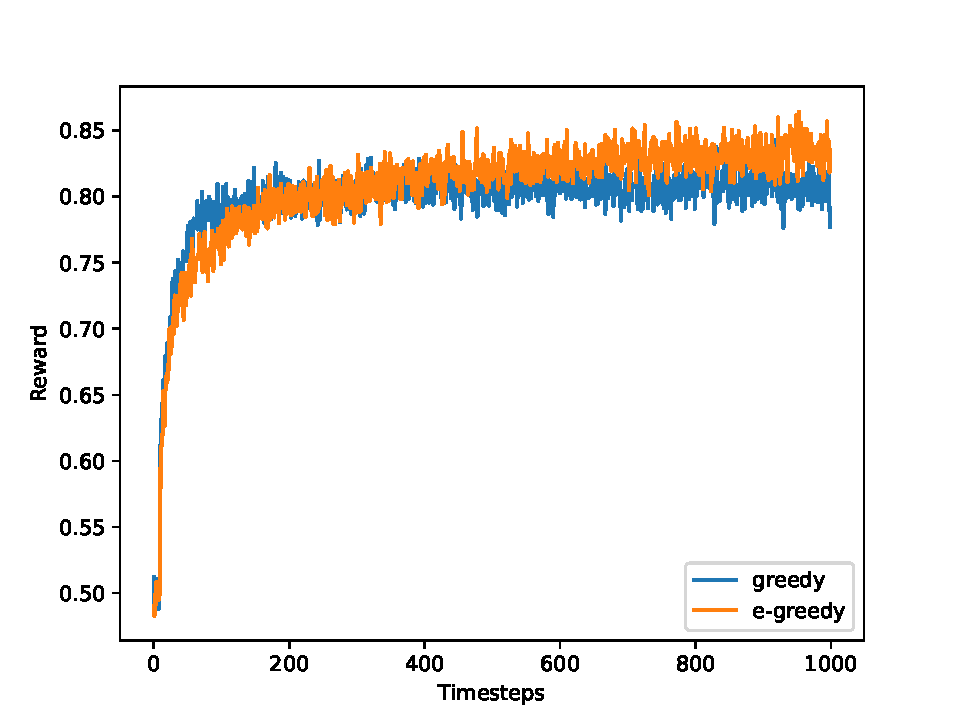
\includegraphics[width=0.95\textwidth]{bandit_strategies.pdf}
\caption{}
\label{fig:strategies}
\end{figure}
\subsection*{Task 2d)}

\begin{itemize}
\item Make the actions not random but according to the Q distribution. Therefore actions which are more likely to actually be the greedy action are chosen more often.
\item Decrease the epsilon over time, so that the agent is more and more exploiting the environment.
\item Make exploration dependent on timesteps, i.e. exploration is more encouraged for larger timesteps. For only ten timesteps maybe just exploit.
\end{itemize}

\end{document}